\documentclass{article}
\usepackage{graphicx} % Required for inserting images
\usepackage{enumitem}
\usepackage{amsmath}
\usepackage[left=2cm,top=2cm,right=2cm,bottom=2cm,bindingoffset=0.4cm]{geometry}
\usepackage[linesnumbered,ruled]{algorithm2e}
\usepackage{pgffor} 
\begin{document}
\begin{center}
\textbf{\Huge Software Design Document}\\
\vspace{70pt}
\textbf{\Large for}\\
\vspace{60pt}
\textbf{\LARGE FastTrack}\\
\vspace{40pt}
\textbf{\large Prepared by}\\
\vspace{30pt}
\textbf{\Large Akhil S Nair (KTE22CS009)}\\
\vspace{30pt}
\textbf{\Large Alwin Philip (KTE22CS012)}\\
\vspace{30pt}
\textbf{\Large Edwin Varkey (KTE22CS028)}\\
\vspace{30pt}
\textbf{\Large Jessin Sunny (KTE22CS036)}\\
\vspace{70pt}
\text{Department of Computer Science and Engineering}\\
\vspace{20pt}
\text{Rajiv Gandhi Institute of Technology,Kottayam}
\end{center}
\newpage
\tableofcontents
\newpage
\begin{figure}
\section{System Design}
\subsection{System Architecture}
\centering
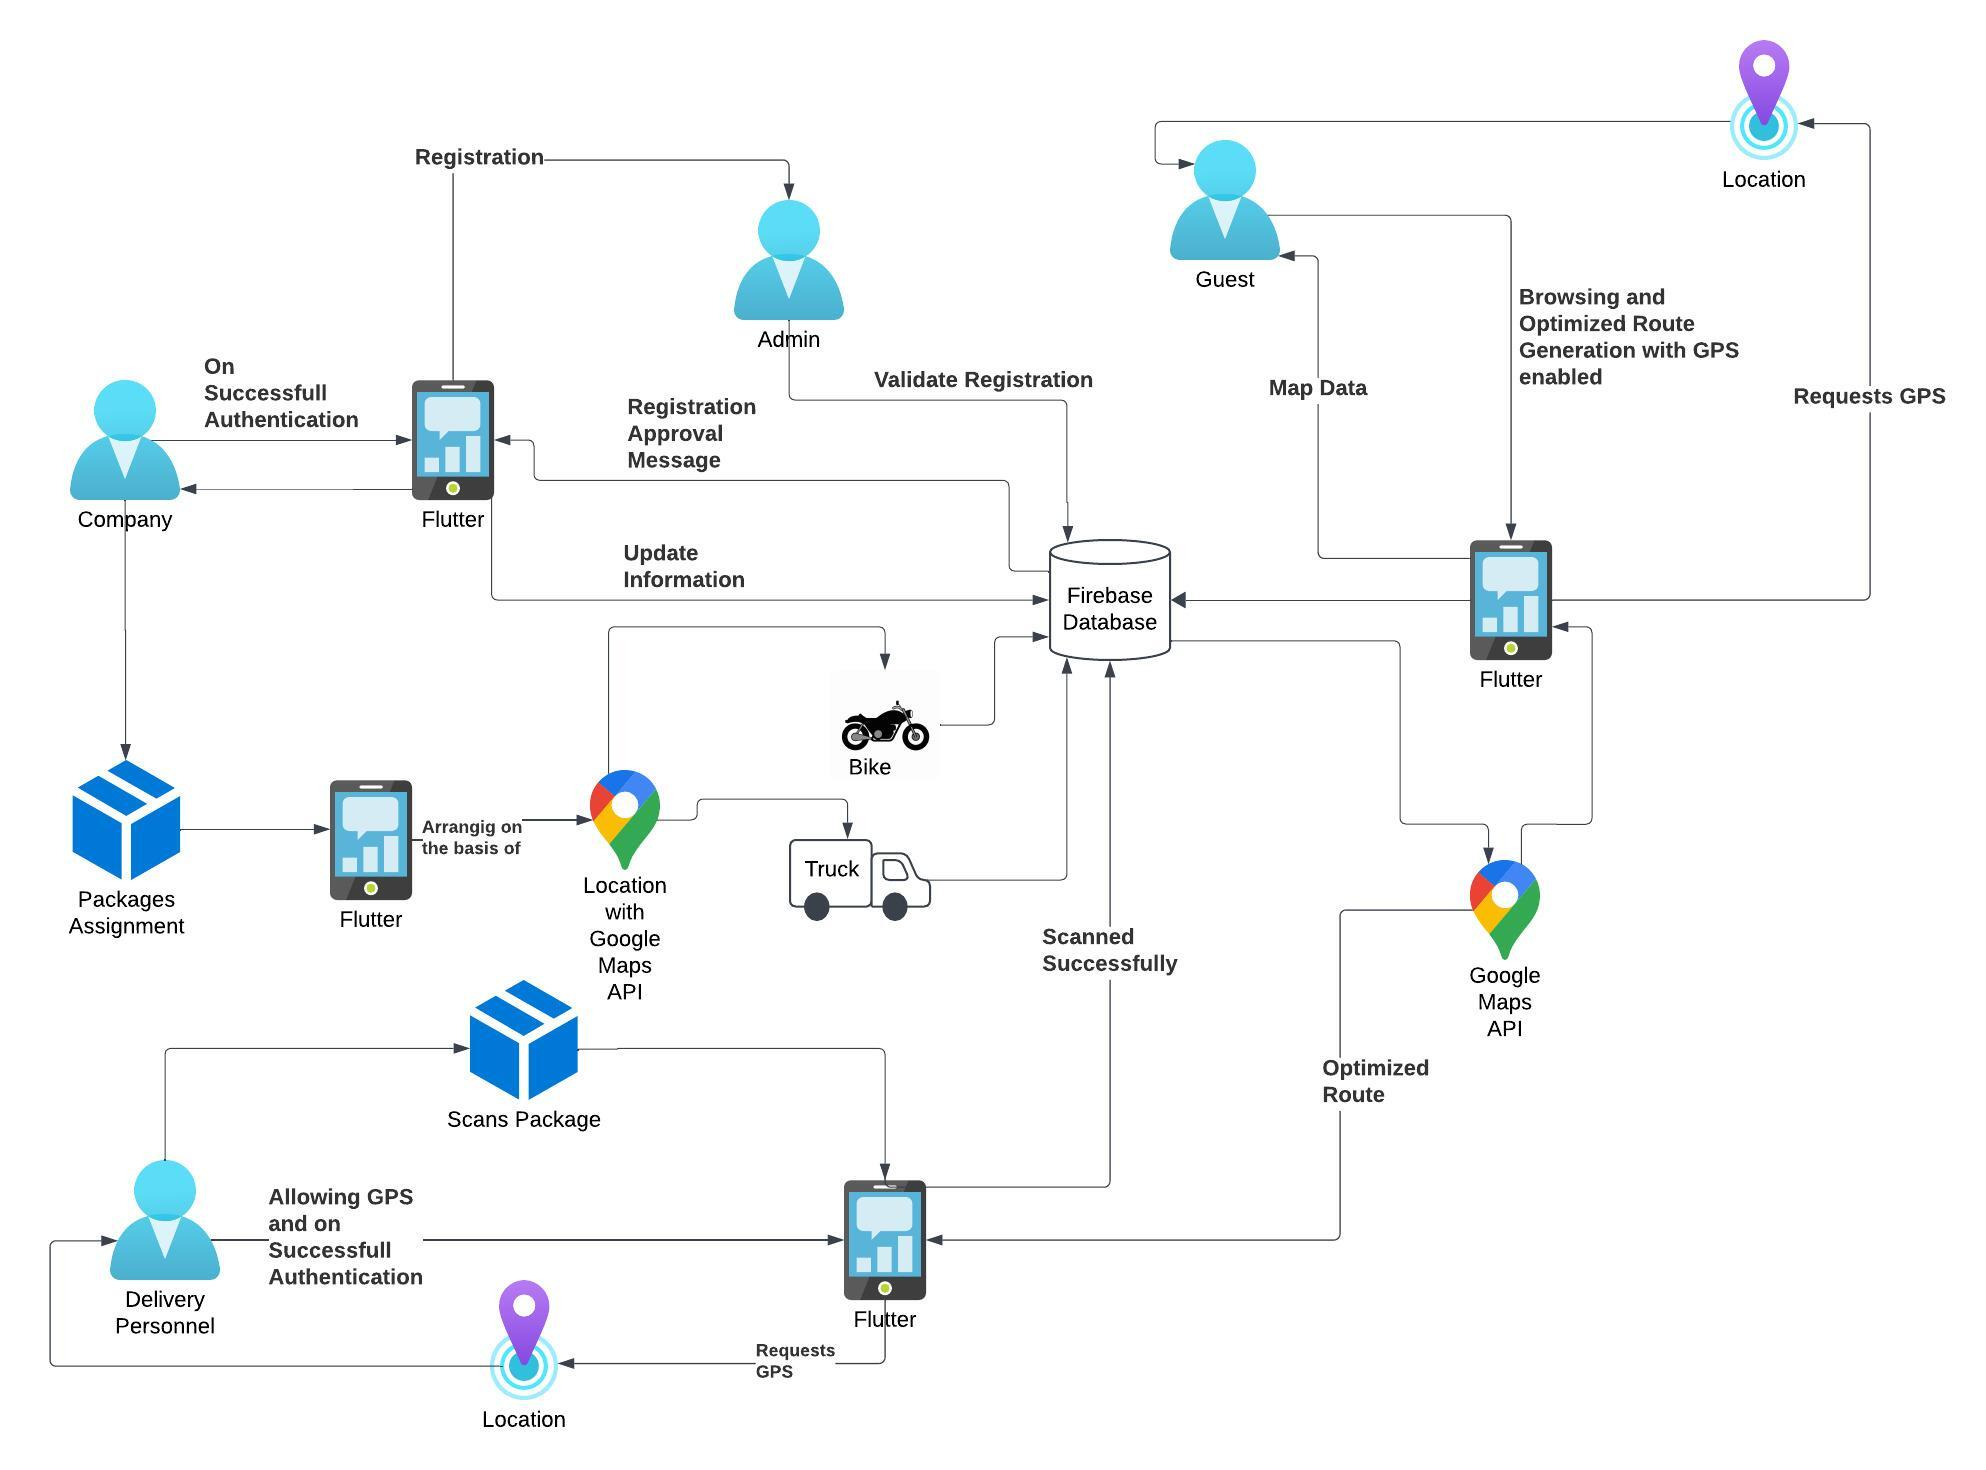
\includegraphics[scale=0.5]{System Architecture.jpeg}
\end{figure}
The figure represents the system architecture for FastTrack, showcasing the interaction between various stakeholders (Admin, Company, Delivery Personnel, and Guest) and technological components.

It uses Flutter for the front-end application, connected to a Firebase Database for centralized data management. The system integrates the Google Maps API for route optimization and location tracking. Key features include company registration and validation by the admin, package assignment and scanning by delivery personnel, and GPS-enabled optimized route generation for efficient deliveries. The architecture also supports different delivery modes like bikes and trucks and allows guests to browse routes or map data.

This system aims to streamline logistics, enhance delivery efficiency, and provide real-time updates for all users involved.
\\\
\newpage

\subsection{USE CASE DIAGRAM}
\vspace{3cm}
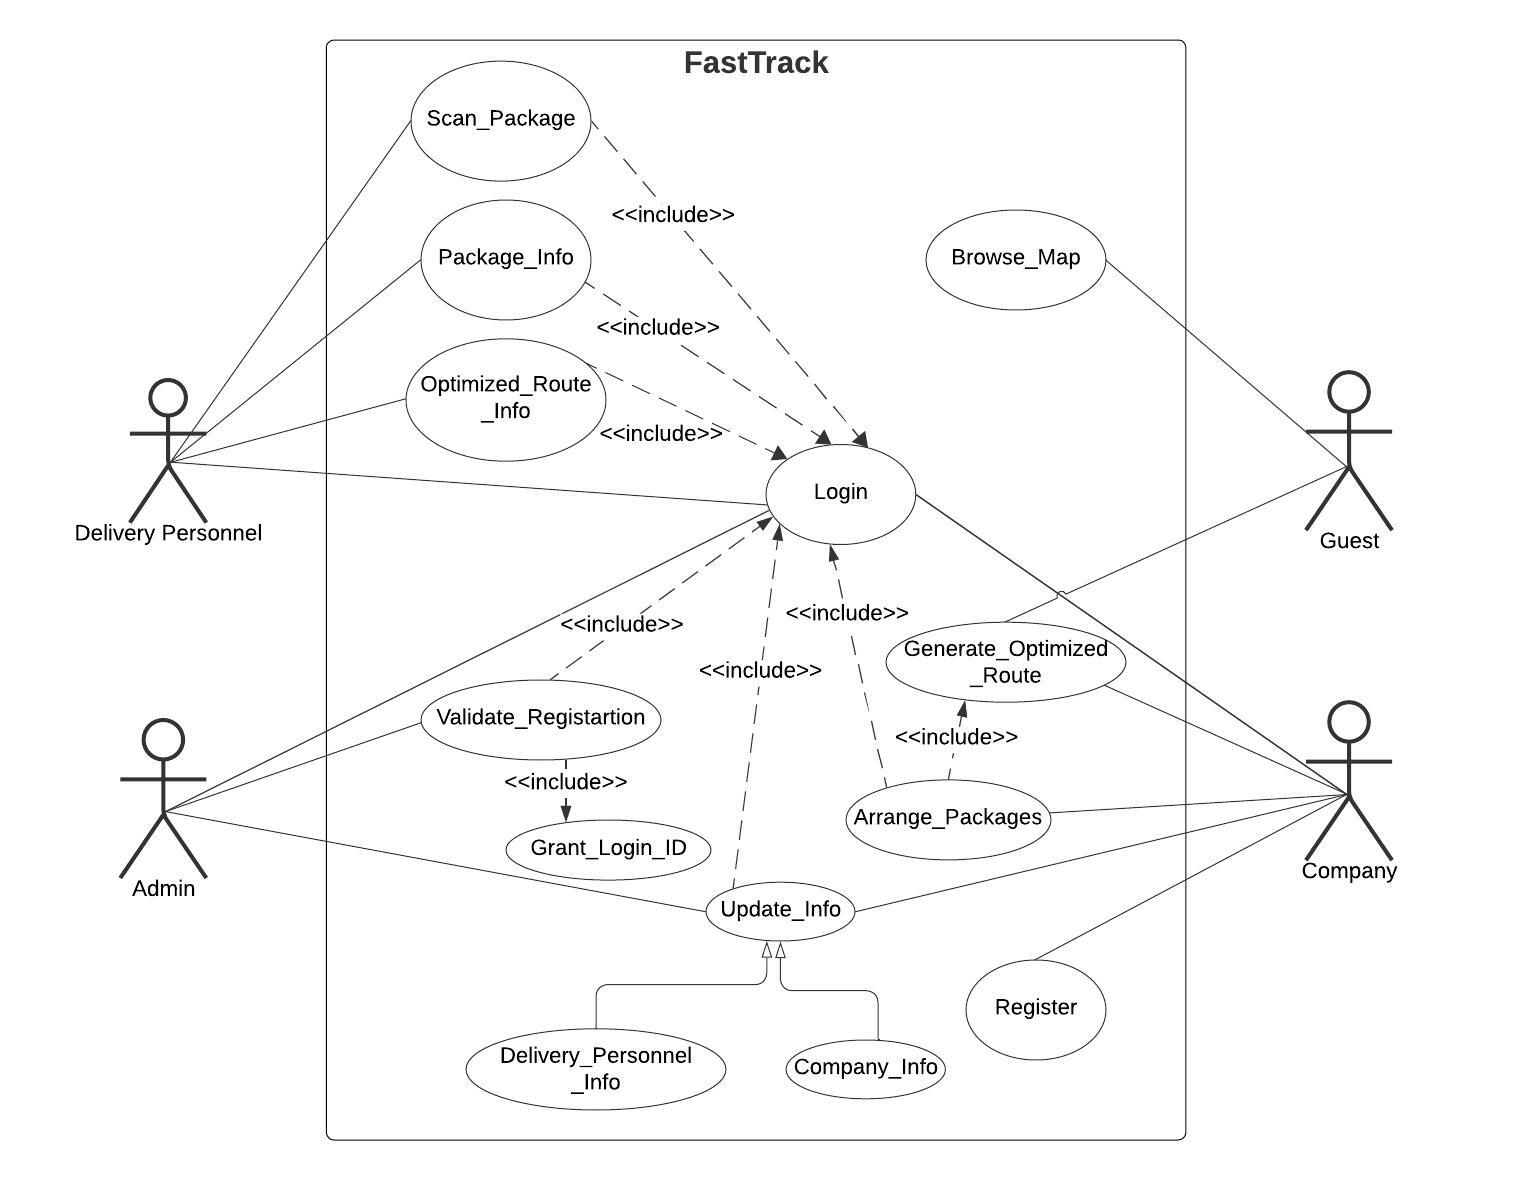
\includegraphics[scale=0.75]{Use case diagram.jpeg}
\newpage

\subsection{User Specific Functionalities}
\begin{itemize}
    \item Delivery Personnel 
    \begin{enumerate}
        \item Login
        \item View package information
        \item Scan packages
        \item Get the optimized route
    \end{enumerate}
    \item Company
    \begin{enumerate}
        \item Register
        \item Login
        \item Updates company and delivery personnel information
        \item Arrange the arrived packages
        \item Generate optimized route for delivery
        \item Locate each delivery personnel current location
    \end{enumerate}
    \item Guest
    \begin{enumerate}
        \item Explore the map
        \item Add destinations
        \item Calculate optimized route
    \end{enumerate}
    \item Admin
    \begin{enumerate}
        \item Login
        \item Validate Registration for Company
        \item Grant company and delivery personnel login ID
        \item Updates company and delivery personnel information      
    \end{enumerate}
\end{itemize}

\newpage
\subsection{Data Flow Diagram}
\subsubsection{0-Level DFD}
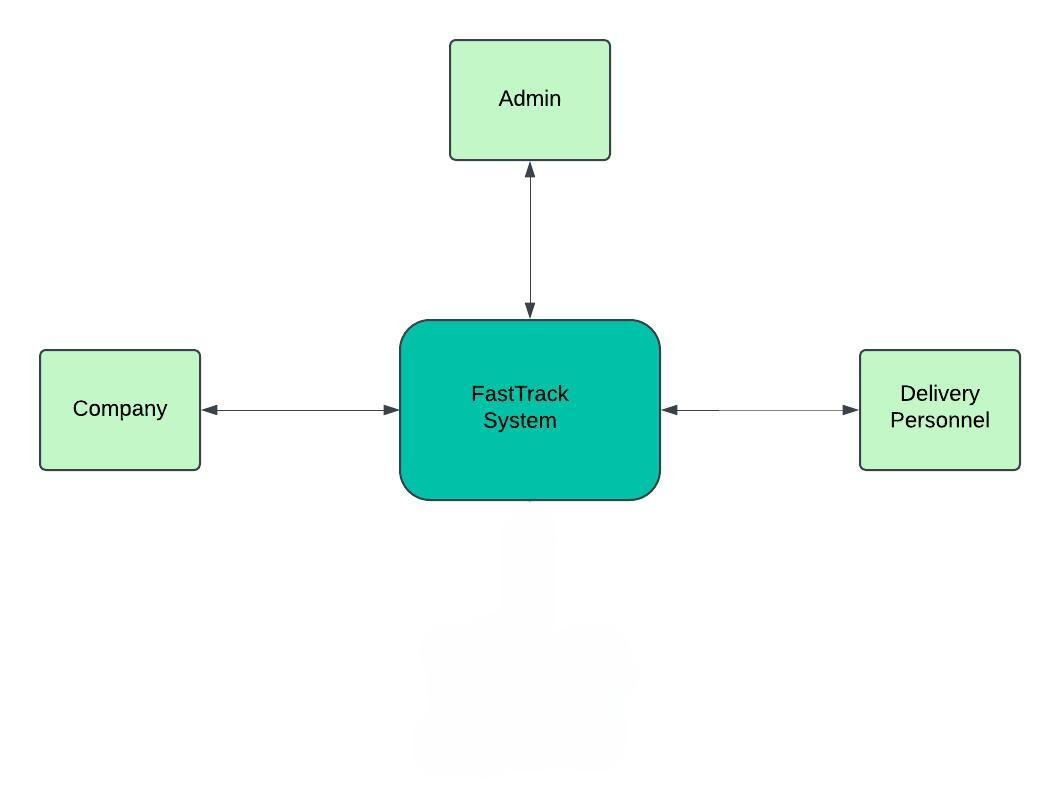
\includegraphics[scale=1.0]{Level 0 Data Flow.jpeg}
\subsubsection{1-Level DFD}
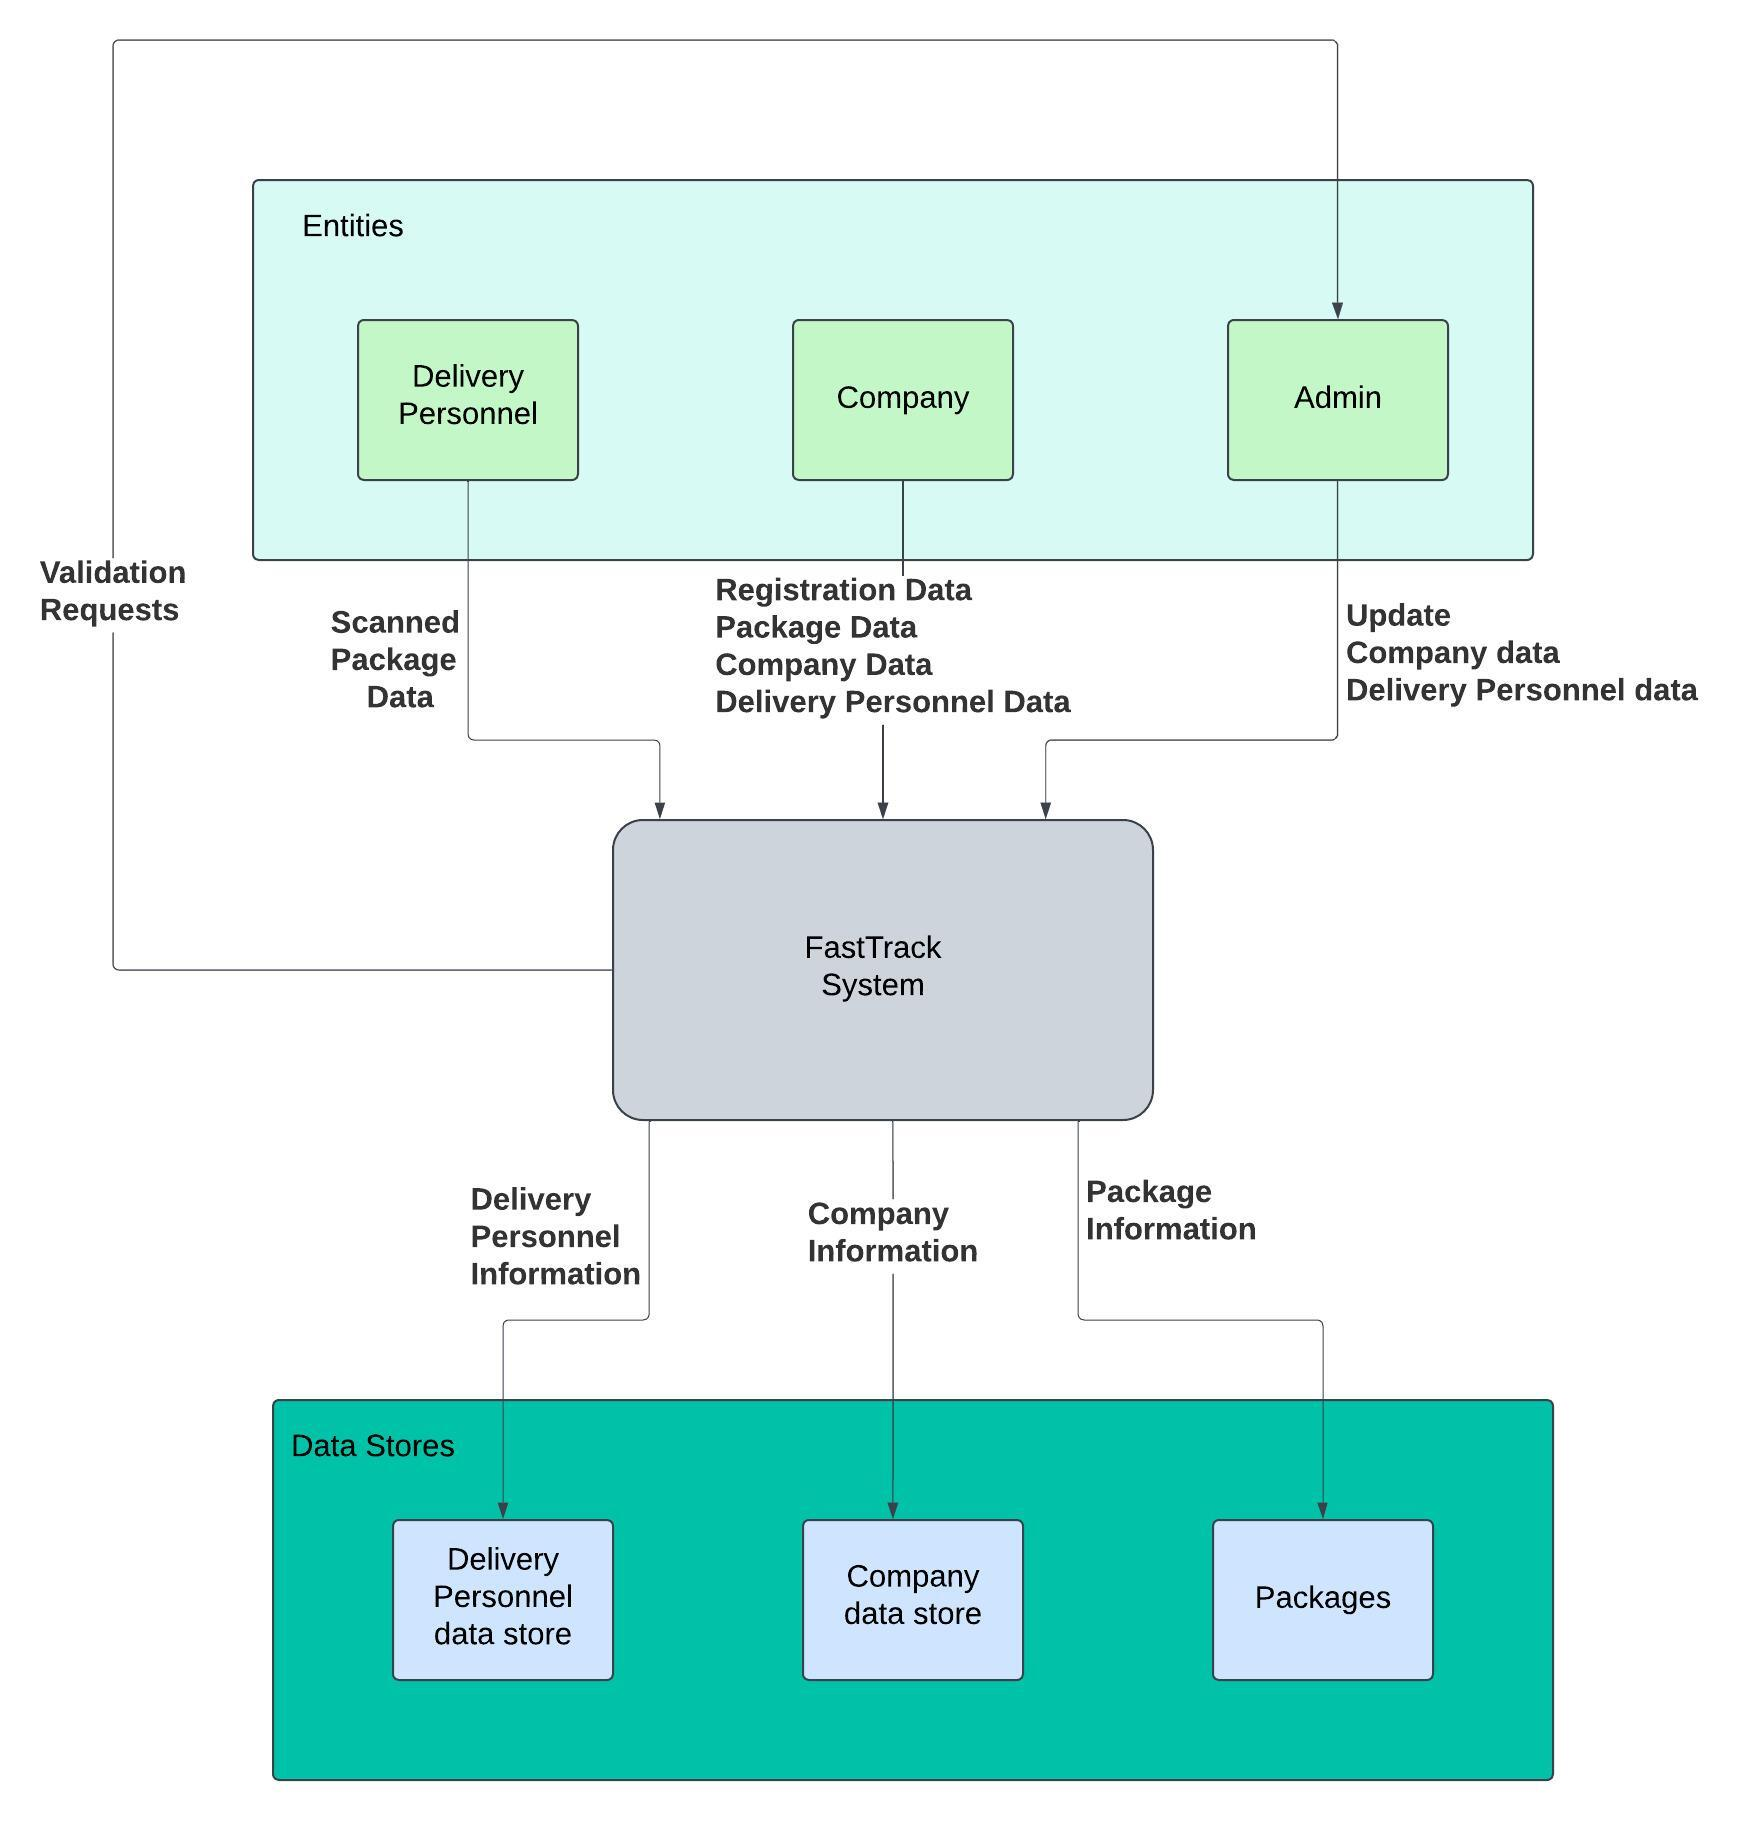
\includegraphics[scale=0.6]{Level 1 Data Flow.jpeg}
\newpage
\section{Detail Design}
\subsection{UI Design}
\vspace{3cm}
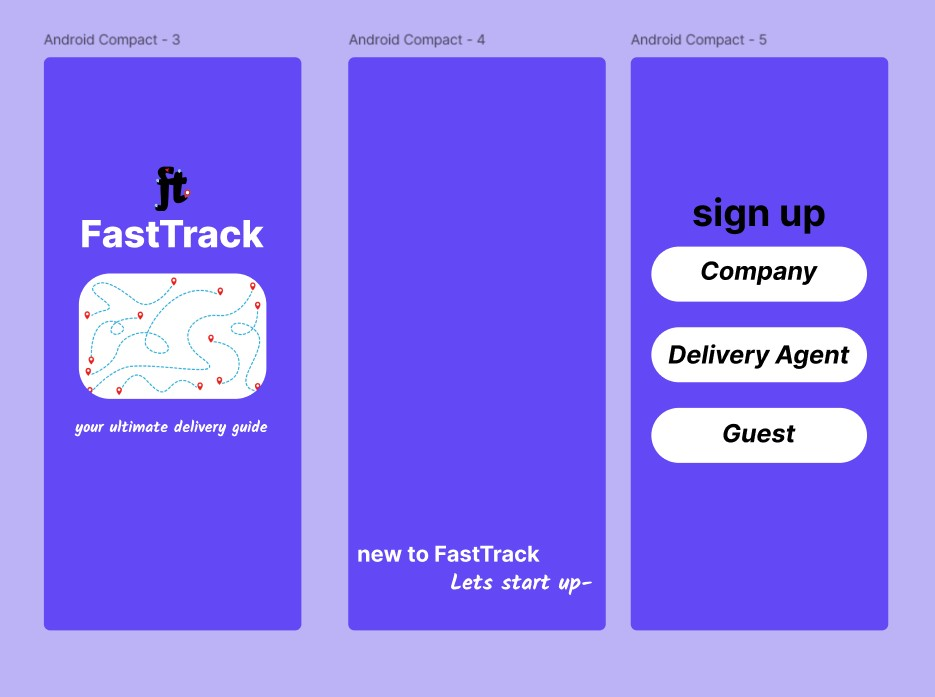
\includegraphics[scale=0.75]{signup.jpg}
\newpage
\vspace*{5cm}
\hspace*{3cm}
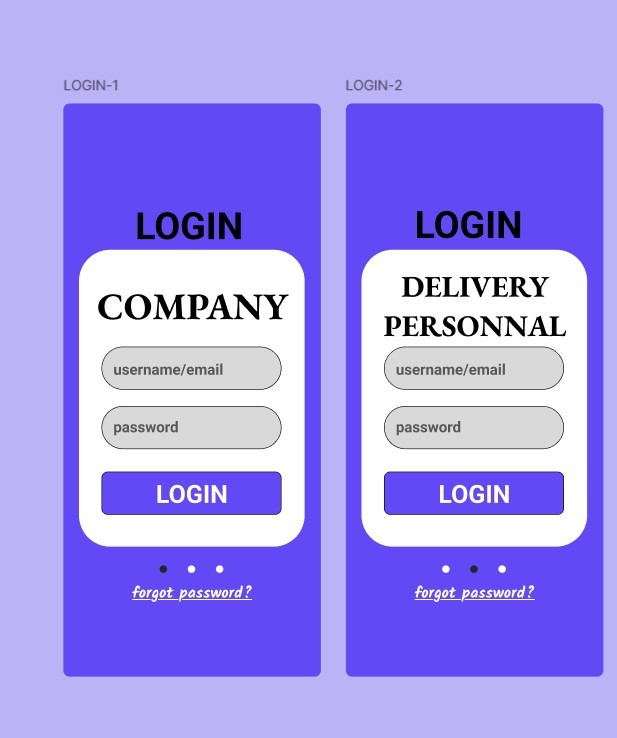
\includegraphics[scale=0.75]{Login.jpg}
\newpage
\hspace*{3cm}
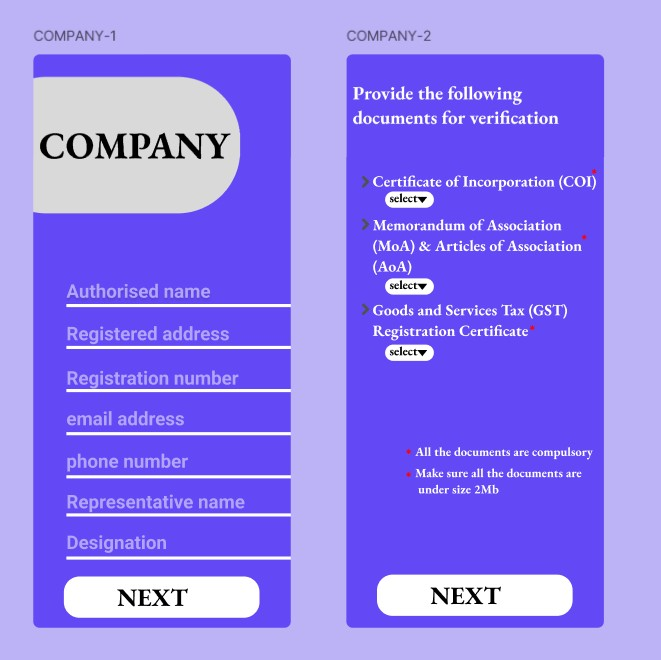
\includegraphics[scale=0.75]{company1.jpg}
\\
\hspace*{3.6cm}
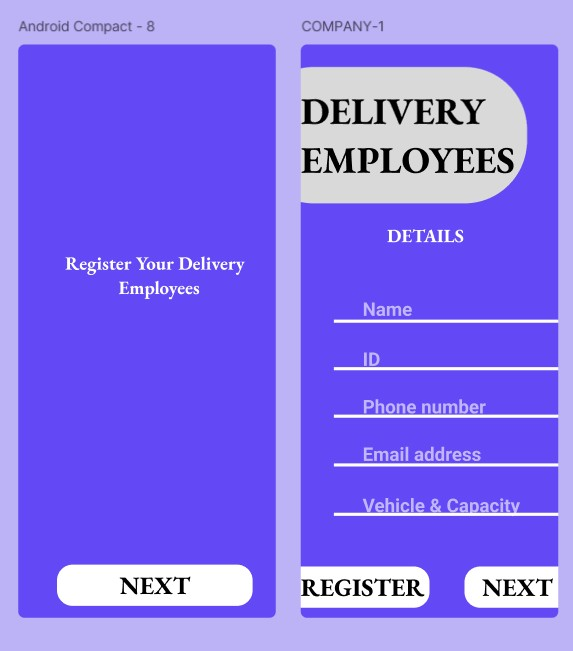
\includegraphics[scale=0.75]{company2.jpg}
\newpage
\vspace*{5cm}
\hspace*{3cm}
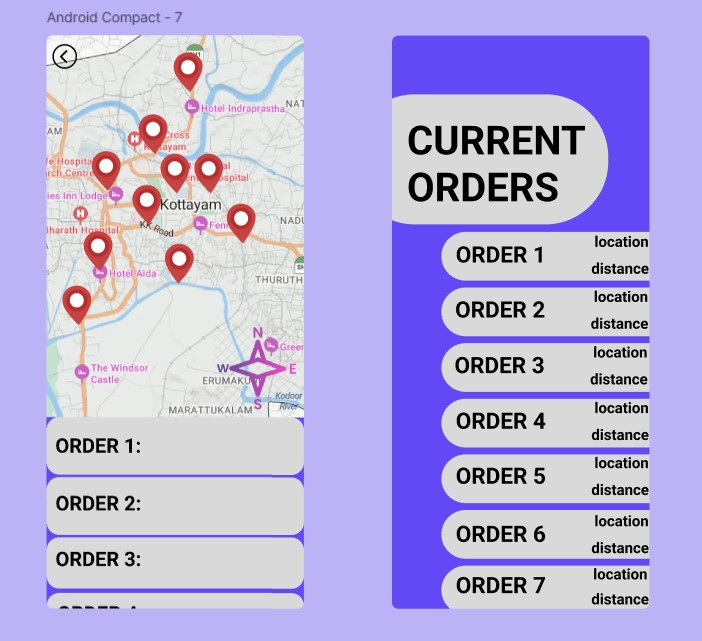
\includegraphics[scale=0.75]{order.jpg}
\newpage
\vspace*{5cm}
\hspace*{3cm}
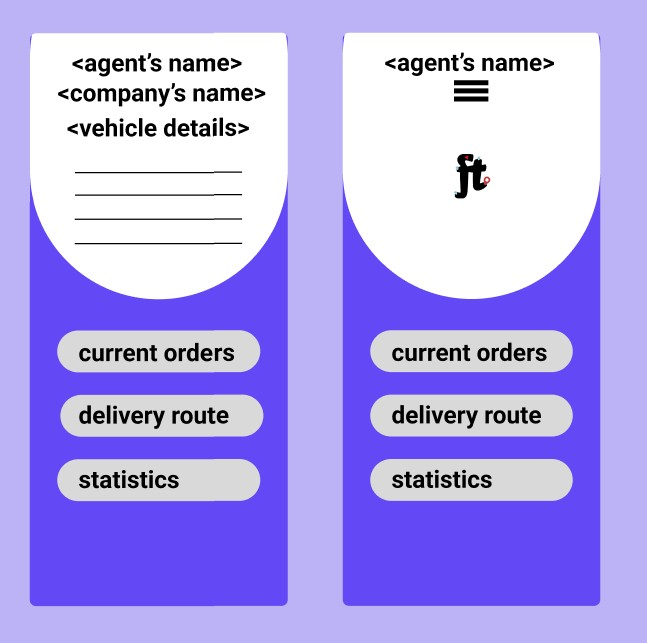
\includegraphics[scale=0.75]{delivery.jpg}
\subsection{ER Diagram}

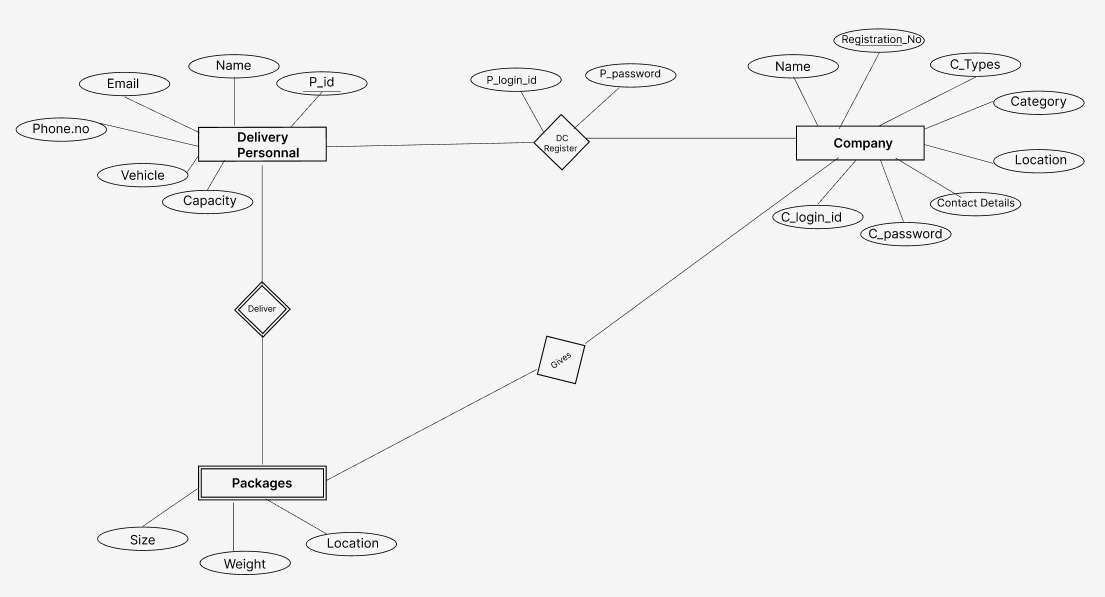
\includegraphics[width=18cm, height=12cm]{ER.jpg}
\newpage

\subsection{Algorithm Design}

\RestyleAlgo{ruled}

%% This is needed if you want to add comments in
%% your algorithm with \Comment
\SetKwComment{Comment}{/* }{ */}

\begin{algorithm}[hbt!]
\caption{Delivery Personnel or Company or Admin Authentication Algorithm}
\SetKwInOut{Input}{Input}
\SetKwInOut{Output}{Output}
\Input{\textnormal{LoginID and Password}}
\Output{\textnormal{Authentication status (Success/Failure message with token if successful)}}
\textnormal{Input the LoginID and Password from the user.}\\
\textnormal{Search for the LoginID in the user database.}\\
\If{the user with the LoginID is found}{
Validate the Password.\\
\If{the Password matches}{
Generate an Authentication Token.\\
Grant access.\\
Display "Authentication Successful".\\
}
\Else{
Display "Invalid Password,Try Again!".
}
}
\Else{
Display "User Not Found". 
}
\end{algorithm}

\begin{algorithm}[H]
\caption{Company Registration}
\SetKwInOut{Input}{Input}
\SetKwInOut{Output}{Output}
\Input{Company Name, Registration Number, Type of Company, Business Category, Address, Contact Details, and Verification Documents}
\Output{Application Number and Validation Status}


Input Company Name, Registration Number, Type of Company, Business Category, Address and Contact Details.\\
Check if the registration number matches the official format using a regular expression.\\
\If{valid}{
    Check if contact details are valid.\\
    \If{valid}{
    Input Certificate of Incorporation, PAN Card and Proof of Address Documents.\\
    \If{Documents uploaded is NULL}{
    Display "Please upload the required documents".
    }
    \Else{
    Generate an application tracking number.\\
    Display "Validation Status: Pending Approval".
    }
    }
    \Else{Display "Invalid Contact Details".}
}
\Else{Display "Invalid Registration Number".}

\end{algorithm}
\begin{algorithm}[H]
\caption{Update Information}
\SetKwInOut{Input}{Input}
\SetKwInOut{Output}{Output}
\Input{
\textnormal{User Role: Admin, Company, or Delivery Personnel \\Update options: Address, Contact Information, Business Category}
}
\Output{ 
    \textnormal{Update Status (Success or Failure)}\\
}
Input User Role: Admin, Company, or Delivery Personnel.
\\
Verify User Login using Algorithm 1.\\
Capture the fields the user wants to update.\\
Access the corresponding database table.\\
Update the relevant fields with the new details.\\
\If{the database update fails}
{
Display "Error updating information. Please try again later".\\
Set Update Status as "Failure".\\
\Else{
Display "Information updated successfully".\\
Set Update Status as "Success".}
}


    
\end{algorithm}
\begin{algorithm}
\caption{Validate Registration}
\SetKwInOut{Input}{Input}
\SetKwInOut{Output}{Output}
\Input{
\textnormal{Certificate of Incooperation, PAN Number and Proof of Address}
}
\Output{Validation status (Valid/Invalid)
}

Input Certificate of Incooperation, PAN Number and Proof of Address.\\
Ensure the Certificate of Incorporation is uploaded.\\
Verify that the PAN Card matches the company name format.\\
Check if the Proof of Address is valid.\\
\If{All validation is done}{
set Validation Status as "Valid".\\
sent LoginID and temporary password to the company's email address.\\
\Else{
set Validation Status as "Invalid".\\
sent a message "Validation Failed due to incorrect document submission" to the company's email address.\\
}
}

\end{algorithm}


\begin{algorithm}
\caption{Scan Package}
\SetKwInOut{Input}{Input}
\SetKwInOut{Output}{Output}
\Input{
\textnormal{Package ID (from the scanned QR code)}
}
\Output{ 
    \textnormal{Scanning Status (Success or Failure) 
}
}
Verify Login using Algorithm 1.\\
Extract the Package ID from the scanned data.\\
Check if the Package ID exists in the system's database.\\
\If{not found}
{
Display "Invalid Package ID. Please scan a valid package".\\
Set Scanning Status as "Failure".\\
}
\Else{
Update the package record in the database\\
Set Scanning Status as "Success."\\
Display "Package successfully scanned and assigned for delivery."\\
}
\end{algorithm}

\begin{algorithm}[H]
\caption{Retrieve Optimized Route After Scanning Packages}
\SetKwInOut{Input}{Input}
\SetKwInOut{Output}{Output}
\Input{
\textnormal{Delivery Personnel ID\\
Scanned Package IDs}
}
\Output{ 
    \textnormal{
    Route Map (Optimized delivery route) or Error Message
}\\
}
Verify Login using Algorithm 1.\\
Ensure all assigned Package IDs are scanned.\\
\If{not all assigned packages are scanned}
{Display "Not all assigned packages are scanned."}
\Else{
Retrieve the Optimized Route generated by the company for this specific set of packages.\\
\If{no route exists}
{Display "Optimized route not available."}

\Else{
Display the Optimized Route Map on the delivery personnel’s interface.
}}
\end{algorithm}

\begin{algorithm}
\caption{Route Optimization with Google Maps API}
\SetKwInOut{Input}{Input}
\SetKwInOut{Output}{Output}
\Input{
\textnormal{Delivery locations (latitude, longitude)}
}
\Output{ 
    \textnormal{Optimized delivery route and total distance}\\
}
Input Delivery Locations as latitude and longitude pairs.\\
Send the locations to Google Maps Distance Matrix API.\\
Receive pairwise distances and travel times between all locations.\\
Set the first location as the starting point.\\
Initialize an empty route list and add the starting location.\\
Optimize Route Using Greedy Algorithm.\\
\While{there are unvisited locations}
{
    Find the nearest unvisited location using the distance matrix\\
    Add the nearest location to $route$\\
    Mark the location as visited\\
}
Add the starting location to the end of the route to complete the cycle.\\
For calculating the total distance, sum the distances between consecutive locations in the route using the distance matrix.\\
Display the optimized route sequence and integrate with Google Maps for visualization.\\
Print the total distance.\\
\end{algorithm}

\begin{algorithm}[hbt!]
\caption{Package Assignment Algorithm}
\SetKwInOut{Input}{Input}
\SetKwInOut{Output}{Output}

\Input{A list of packages (with attributes: destination, weight, size, priority, deadline) and a list of delivery boys (with attributes: max\_weight, max\_volume, max\_hours).}
\Output{Assignment of packages to delivery boys, ensuring load balancing and prioritization.}

Create a dictionary `destination\_groups` to store packages grouped by their destination.\\
\ForEach{package in the list of packages}{
    Add the package to the corresponding group in `destination\_groups`.
}

\ForEach{destination in `destination\_groups`}{
    Sort the packages in the group by priority (ascending) and deadline (ascending).
}

Initialize an empty list `sorted\_packages`.\\
\ForEach{group in `destination\_groups`}{
    Append all packages from the group to `sorted\_packages`.
}

Initialize delivery\_boys with current\_weight and current\_volume set to 0.\\
\ForEach{package in sorted\_packages}{
    Sort delivery\_boys by (current\_weight + current\_volume) in ascending order.\\
    \ForEach{boy in delivery\_boys}{
        \If{(boy.current\_weight + package.weight $\leq$ boy.max\_weight) \textbf{and} \\
            (boy.current\_volume + package.size $\leq$ boy.max\_volume)}{
            Append package to boy.assigned\_packages.\\
            Update boy.current\_weight $\gets$ boy.current\_weight + package.weight.\\
            Update boy.current\_volume $\gets$ boy.current\_volume + package.size.\\
            \textbf{break} \Comment{Package assigned, move to the next package.}
        }
    }
}
\ForEach{boy in delivery\_boys}
{
Print the number of packages assigned to the boy.\\
\ForEach{package assigned to the boy}
{
Print the package's destination, weight, and size.\\
}
}
\end{algorithm}

\end{document}
